%%%%%%%%%%%%%%%%%%%%%%%%%%%%%%%%%%%%%%%%%%%%%%%%%%%
%% P3: Phenomenology of Particle Physics                         
%%
%% Author:  André Rubbia                   		 
%%
%% Figure 13.8 Measurements of the forward--backward asymmetry.
%%
%% This work is licensed under the Creative Commons Attribution 4.0 International License. 
%% To view a copy of this license, visit http://creativecommons.org/licenses/by/4.0/ or 
%% send a letter to Creative Commons, PO Box 1866, Mountain View, CA 94042, USA.
%%
%%%%%%%%%%%%%%%%%%%%%%%%%%%%%%%%%%%%%%%%%%%%%%%%%%%

\documentclass[a4paper,10pt]{article}

\usepackage[T1]{fontenc}
\usepackage[utf8]{inputenc}
\usepackage{lmodern}
\usepackage[labelfont=bf]{caption}
\usepackage{upgreek}

\usepackage{tikz}
\usepackage{pgfplots}
\pgfplotsset{compat=1.17}
\usepgfplotslibrary{ternary}
\usepgfplotslibrary{fillbetween}
\usepgfplotslibrary{external}

\usepackage{braket}

\def\d{\mathrm{d}}

\pgfkeys{/pgf/number format/.cd,1000 sep={}}

\begin{document}

%%%%%%%%%%%%%%%%% FIGURE %%%%%%%%%%%%%%%%%%%%%%%%%%%%%%%%%%
\begin{figure}[htb]
\begin{center}
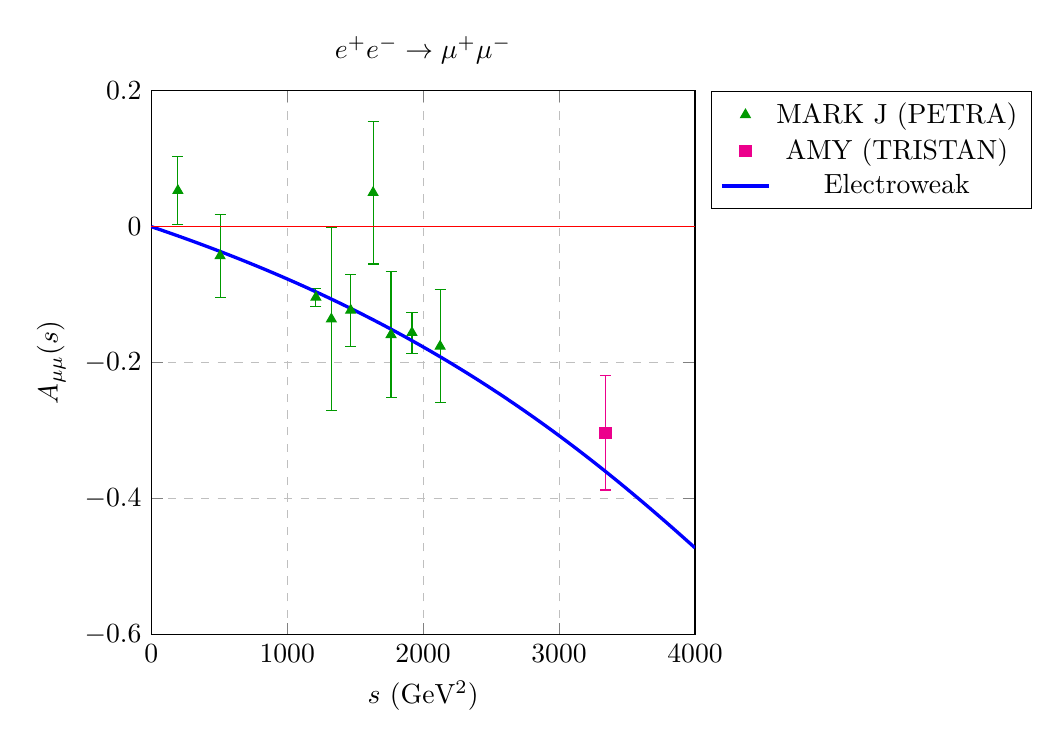
\begin{tikzpicture}[scale=1.]
\begin{axis}[
    width=0.7\textwidth,
    height=0.7\textwidth,
    title={$e^+e^-\rightarrow \mu^+\mu^-$},
    xlabel={$s$~(GeV$^2$)},
    ylabel={$A_{\mu\mu}(s)$},
    xmin=0, xmax=4000,
    ymin=-0.6, ymax=0.2,
	legend style={legend pos = outer north east},
    	ymajorgrids=true,
    	xmajorgrids=true,
    grid style=dashed,
]


%% MarkJ R_mumu 10.1103/PhysRevD.38.2665
\addplot[
    color=green!60!black,
    only marks,
    mark = triangle*,
    error bars/.cd,
    y dir=both, y explicit
    ]
    coordinates {
    % 14 GeV
 ( 196 , 0.053 )+-(0, 0.05 )
   % 22.5
( 506.25 , -0.043 )+-(0, 0.061 )
  % 34.8
  ( 1211.16 , -0.104 )+-(0, 0.013 )
  % 36.4
  ( 1325.0,  -0.136)+-(0, 0.135)
  % 38.3
  ( 1467, -0.123)+-(0, 0.053)
  % 40.4
  ( 1632, 0.05)+-(0, 0.105)
  % 42.0
  ( 1764, -0.159)+-(0, 0.093)
  % 43.8
  (  1918, -0.156)+-(0, 0.03)
  % 46.1
  ( 2125, -0.176)+-(0, 0.083)
%( 1584.0399999999997 , 1.01 )+-(0, 0.06403124237432849 )
%( 1989.16 , 0.99 )+-(0, 0.0565685424949238 )
};

%
% AMY A_mumu 10.1016/0370-2693(94)90967-9 Phys.Lett.B 331 (1994) 227-235
\addplot[
    color=magenta,
    only marks,
    mark = square*,
    error bars/.cd,
    y dir=both, y explicit
    ]
    coordinates {
% 52
%( 2704.0 , 1.02 )+-(0, 0.14 )
% 55
%( 3025.0 , 0.80 )+-(0, 0.16 )
% 56
%( 3136.0 , 1.09 )+-(0, 0.12 )
% 57.8
( 3341 , -0.303)+-(0, 0.0844334 )
};


%% GSW
\addplot[
    color=blue,very thick,smooth
    ]
    coordinates {
( 0, 0.0 )
( 50, -0.0034032489918318113 )
( 100, -0.00684883412337216 )
( 150, -0.010337437722454374 )
( 200, -0.013869753568402752 )
( 250, -0.01744648699240834 )
( 300, -0.02106835496958843 )
( 350, -0.02473608620178148 )
( 400, -0.028450421190053164 )
( 450, -0.03221211229580772 )
( 500, -0.03602192378931152 )
( 550, -0.039880631884341905 )
( 600, -0.043789024757573375 )
( 650, -0.04774790255120559 )
( 700, -0.05175807735722175 )
( 750, -0.05582037318154139 )
( 800, -0.059935625886199065 )
( 850, -0.06410468310753692 )
( 900, -0.06832840414824702 )
( 950, -0.07260765984093484 )
( 1000, -0.07694333238070004 )
( 1050, -0.08133631512404249 )
( 1100, -0.08578751235120127 )
( 1150, -0.09029783898881684 )
( 1200, -0.094868220289579 )
( 1250, -0.09949959146527432 )
( 1300, -0.10419289726938455 )
( 1350, -0.10894909152510553 )
( 1400, -0.11376913659435475 )
( 1450, -0.1186540027830147 )
( 1500, -0.12360466767731534 )
( 1550, -0.1286221154058937 )
( 1600, -0.1337073358216761 )
( 1650, -0.13886132359731462 )
( 1700, -0.14408507722746253 )
( 1750, -0.14937959793070366 )
( 1800, -0.15474588844344594 )
( 1850, -0.160184951697555 )
( 1900, -0.16569778937293647 )
( 1950, -0.1712854003156706 )
( 2000, -0.17694877881166435 )
( 2050, -0.18268891270510673 )
( 2100, -0.18850678135029622 )
( 2150, -0.19440335338464906 )
( 2200, -0.20037958430989483 )
( 2250, -0.20643641386762215 )
( 2300, -0.21257476319444304 )
( 2350, -0.21879553174111133 )
( 2400, -0.22509959393894505 )
( 2450, -0.23148779559587385 )
( 2500, -0.237960950003356 )
( 2550, -0.24451983373428676 )
( 2600, -0.25116518211085237 )
( 2650, -0.257897684320075 )
( 2700, -0.26471797815354065 )
( 2750, -0.2716266443465179 )
( 2800, -0.27862420049035386 )
( 2850, -0.2857110944906889 )
( 2900, -0.2928876975426691 )
( 2950, -0.30015429659296106 )
( 3000, -0.3075110862570053 )
( 3050, -0.31495816015858497 )
( 3100, -0.3224955016574675 )
( 3150, -0.3301229739296009 )
( 3200, -0.33784030936314446 )
( 3250, -0.3456470982325151 )
( 3300, -0.35354277661165445 )
( 3350, -0.3615266134869124 )
( 3400, -0.36959769702933903 )
( 3450, -0.37775491998581884 )
( 3500, -0.38599696414842694 )
( 3550, -0.3943222838616933 )
( 3600, -0.40272908852819816 )
( 3650, -0.4112153240741561 )
( 3700, -0.4197786533384764 )
( 3750, -0.4284164353512923 )
( 3800, -0.4371257034712476 )
( 3850, -0.44590314235502587 )
( 3900, -0.4547450637378328 )
( 3950, -0.46364738100993297 )
( 4000, -0.47260558258205354 )
};

\addplot [red,domain=0:4000, samples=75] {0};

    \legend{
     MARK J (PETRA),
     AMY (TRISTAN),
	Electroweak
 	}
\end{axis}

\end{tikzpicture}

\caption{Measurements of the forward--backward asymmetry $A_{\mu\mu}$ in the reaction $e^+e^-\rightarrow\mu^+\mu^-$
from Mark-J and
AMY,
plotted as a function of the center-of-mass energy squared $s$. The thick line labeled ``Electroweak'' corresponds to the prediction of the electroweak theory, while
the horizontal line at zero would be the case with only QED. }
\end{center}
\end{figure}
%%%%%%%%%%%%%%%%% END FIGURE %%%%%%%%%%%%%%%%%%%%%%%%%%%%%%
%

\end{document}
